\renewcommand{\theHchapter}{A\arabic{chapter}}
\appchapter{CHOICE OF THE BRANCH CUT FOR THE COMPLEX-VALUED SQUARE ROOT FUNCTION\label{appBranchCut}}

Here I consider a~general case of a~wave of a~form
\begin{equation}
\label{eq:waveA}
u(x,y,z,t) = u_0 e^{ik_xx+ik_zz-i\omega t}
\end{equation}
propagating in a~homogeneous and isotropic medium in the~semispace $z>0$ bounded by an~interface $z=0$.
Suppose the~dispersion of the~wave is parabolic,
\begin{equation}
\label{eq:dispA}
k_x^2+k_z^2 = \frac{\omega^2}{c_{ph}^2},
\end{equation}
with $c_{ph}$ being the~phase velocity of the~wave.

Now, if the~value of the~$x$-component of the~wave vector, $k_x$, is determined by the~physical process developing in the~medium, one can find the~$z$-component of the~wave vector to be
\begin{equation}
\label{eq:dispkzA}
k_z = \sqrt{\frac{\omega^2}{c_{ph}^2}-k_x^2}.
\end{equation}

If the~value of $k_x$ is real and $k_x < \omega/c_{ph}$, the~value of $k_z$ is then also real, and the~wave \cref{eq:waveA} is a~simple plane wave running in the~direction of $\textbf{k} = (k_x,0,k_z)$.
In the~case of $k_x > \omega/c_{ph}$ the~value of $k_y$ is purely imaginary, $k_z = i\sqrt{k_x^2-\omega^2/c_{ph}^2} = i\kappa_z$, $\kappa_z>0$, which is typical for guided modes that propagate along an~interface in the~$x$-direction and decay in the~perpendicular direction into the~medium:
\begin{equation*}
u(x,y,z,t) = u_0 e^{ik_xx-\kappa_zz-i\omega t}.
\end{equation*}

There are, however, two other possible wave behaviors that are described by the complex-valued $k_x$ and therefore require special attention.
First of all, the~energy carried with the~wave can only dissipate, which corresponds to $\im k_x > 0$, and the~case of $\im k_x < 0$ does not have any physical sense.
This implies that $k_x$ lies in the~first quadrant of the~complex plane, and therefore $k_z^2 = \omega^2/c_{ph}^2-k_x^2$ is in either third or fourth quadrants.
On the~other hand, the~relationship \cref{eq:dispA} dictates that the~signs of the~real and imaginary parts of $k_z$ be opposite (with $k_z$ in the~second or fourth quadrants), otherwise it cannot be satisfied for any given purely real $\omega$ and complex $k_x$ with both $\re k_x > 0$ and $\im k_x > 0$.

For the~positive values of $\re k_z^2$, i.e., when $\re\left(\omega^2/c_{ph}^2-k_x^2\right) > 0$, the~correct behavior of the~wave is the~radiative one, with $\re k_z > 0$, so the~square root should map the~values of $k_z^2$ from the~fourth quadrant into the~fourth quadrant.
Note that $\im k_z > 0$ in this case, which formally means an~exponential growth of the~wave amplitude away from the~interface.
However, the~amplitude decay along the~$x$-axis "compensates" for the~growth along the~$z$-axis \cite{maradudin1,ingerbrigsten,lim}, and, in fact, it can be shown that such a~wave propagates with a~constant amplitude along the~direction of $\mathbf{k'} = (\re k_x,0,\re k_z)$.
This is a~clear manifestation of the~radiative behavior since the~energy of the~wave is not being transmitted along the~interface but is rather carried away at an~angle from it.

For the~negative values of $\re k_z^2$, the~wave must be nonradiative \cite{maradudin2,maradudin3}, with positive $\im k_z$ providing the~exponential decay away from the~interface, and the~corresponding mapping for the~square root function is from the~third into the~second quadrant.

One possibility to satisfy all the~conditions outlined above is to define the~complex-valued square root function with the~branch cut along the~negative imaginary axis.
%
Alternatively, one can use the~conventional square-root function (with the~branch cut along the~negative real axis) and, instead, explicitly specify the~sign ("$+$" or "$-$") in front of the~square root in \cref{eq:dispkzA} in each case.



\appchapter{CALCULATION OF FOURIER TRANSFORMS FOR PROPAGATING AND LEAKY RAYLEIGH EIGENMODES}\label{appRayleigh}

Consider the~integral
\begin{equation}
\label{eq:fourierA}
\CF(k, \varkappa)~=~\frac{e^{\varkappa d/2}}{2}\left(\int\limits_{-\infty}^{-d/2}e^{-ikz+\varkappa z}dz + \int\limits_{+d/2}^{+\infty}e^{-ikz-\varkappa z}dz\right)
\end{equation}
which arises when the~Fourier transforms of \cref{eq:B5Rayleigh}-\cref{eq:B6Rayleigh} are calculated.
If the~parameter $\varkappa$ describes the~propagating Rayleigh eigenmode, i.e., if $\re \varkappa > 0$ and $\im \varkappa = 0$, the~calculation of \cref{eq:fourierA} is trivial:
\begin{align}
\CF(k, \varkappa)~&=~\frac{e^{\varkappa d/2}}{2}\left(\int\limits_{-\infty}^{-d/2}e^{-ikz+\varkappa z}dz + \int\limits_{+d/2}^{+\infty}e^{-ikz-\varkappa z}dz\right)~=\\
&=~\frac{e^{\varkappa d/2}}{2}\int\limits_{+d/2}^{+\infty}\left(e^{+ikz-\varkappa z}+e^{-ikz-\varkappa z}\right)dz~= \notag\\
&=~\frac{e^{\varkappa d/2}}{2}\left(\frac{e^{(ik-\varkappa)d/2}}{\varkappa-ik}+\frac{e^{(-ik-\varkappa)d/2}}{\varkappa+ik}\right)~= \notag\\
&=~\frac{1}{k^2+\varkappa^2}\left(\varkappa \cos\frac{kd}{2}-k\sin\frac{kd}{2}\right). \notag
\end{align}

However, for the~leaky Rayleigh eigenmode with $\re\varkappa < 0$ and $\im\varkappa < 0$ the~integral \cref{eq:fourierA} diverges.
Its value can be written as a~limit
\begin{equation}
\CF(k, \varkappa)~=~\frac{e^{\varkappa d/2}}{2}\left(\frac{e^{(ik-\varkappa)d/2}}{\varkappa-ik}+\frac{e^{(-ik-\varkappa)d/2}}{\varkappa+ik}\right) - \lim\limits_{Z\rightarrow +\infty}\frac{e^{\varkappa d/2}}{2}\left(\frac{e^{(ik-\varkappa)Z/2}}{\varkappa-ik}+\frac{e^{(-ik-\varkappa)Z/2}}{\varkappa+ik}\right).
\end{equation}

It was shown in \cite{jia} that the~divergence can be avoided with the~introduction of perfectly matched layers (PMLs) in the~regions $|z| > L$, where $L$ is a~characteristic distance beyond which the~physical processes are of no interest.
In the~problem of sound transmission through a~fluid channel between two elastic plates, $L$ could be the~size of the~actual plates in the~direction away from the~channel.
Within the~PML the~signal undergoes fast attenuation, and the~PML behavior is typically modeled by a~complex coordinate transform.
Namely, the~integral in the~original limits is split into two parts
\begin{equation}
\int\limits_{d/2}^{+\infty}f(z)dz \rightarrow \int\limits_{d/2}^{L}f(z)dz + \int\limits_{L}^{+\infty}f(z')g(z')dz',
\end{equation}
where the~attenuation in the~PML is added by the~factor $g(z')$, and the~latter integral must be identical to the~integral along the~line in the~complex plane $z$:
\begin{equation}
\int\limits_{L}^{+\infty}f(z')g(z')dz' \equiv \int\limits_{L}^{L+(1+i\alpha)\infty}f(z)dz.
\end{equation}

The~integrands in \cref{eq:fourierA} are analytical functions, so the~contour integral
\begin{equation}
\CF(k, \varkappa)~=~\frac{e^{\varkappa d/2}}{2}\int\limits_{+d/2}^{L+(1+i\alpha)\infty}\left(e^{+ikz-\varkappa z}+e^{-ikz-\varkappa z}\right)dz
\end{equation}
is evaluated to
\begin{equation}
\label{eq:limitA}
\CF(k, \varkappa)~=~\frac{e^{\varkappa d/2}}{2}\left(\frac{e^{(ik-\varkappa)d/2}}{\varkappa-ik}+\frac{e^{(-ik-\varkappa)d/2}}{\varkappa+ik}\right) - \lim\limits_{Z\rightarrow L+(1+i\alpha)\infty}\frac{e^{\varkappa d/2}}{2}\left(\frac{e^{(ik-\varkappa)Z/2}}{\varkappa-ik}+\frac{e^{(-ik-\varkappa)Z/2}}{\varkappa+ik}\right).
\end{equation}
The~value of $\alpha$, which characterizes the~PML, must be chosen to guarantee the~finite value of the~limit in the~latter expression.

For $k \ge 0$ and $\alpha > \left|\re\varkappa/\im\varkappa\right|$ the~limit in \cref{eq:limitA} is zero and
\begin{equation}
\CF(k, \varkappa)~=~\frac{1}{k^2+\varkappa^2}\left(\varkappa \cos\frac{kd}{2}-k\sin\frac{kd}{2}\right).
\end{equation}

The~final result is the~same for negative values of $k$ as well, as the~function $\CF(k,\varkappa)$ is even with respect to its first argument.



\appchapter{GRAF'S ADDITION THEOREM}\label{appGrafTheorem}

Let there be a~triangle formed by the~vectors $\mathbf{r}_j$, $\mathbf{r}_l$, and $\mathbf{R}_{jl} = \mathbf{r}_j - \mathbf{r}_l$ as shown in the~\cref{fig:grafB}.
Suppose that $\mathbf{r}_l$ has the~coordinates $\left(r_l, \varphi_l\right)$ in the~polar coordinate system with the~origin in $O_l$, while $\mathbf{r}_j = \left(r_j, \varphi_j\right)$ and $\mathbf{R}_{jl} = \left(R_{jl}, \vartheta_{jl}\right)$ in the~polar coordinate system with the~origin in $O_j$.

\begin{figure}
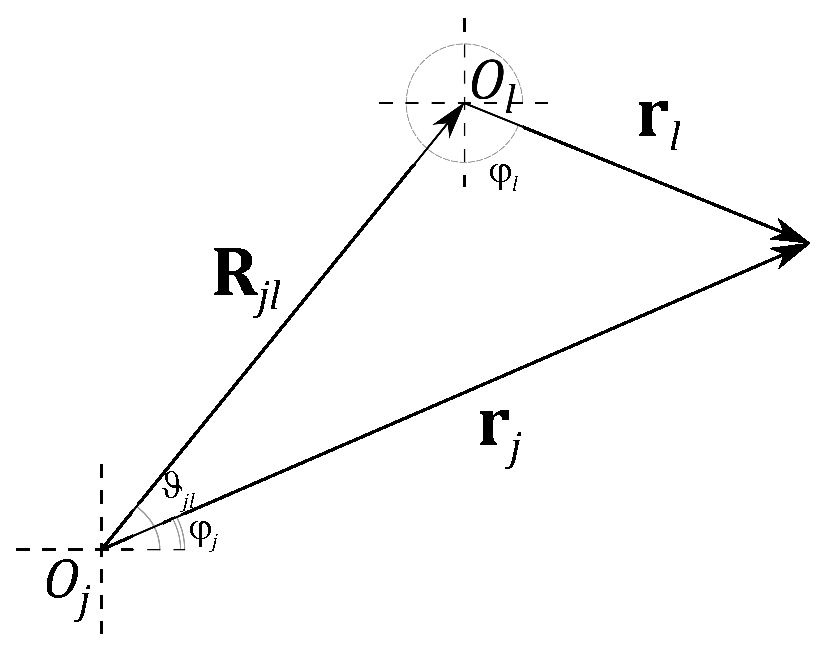
\includegraphics[scale=1]{grafs.eps}
\caption{The~three vectors $\mathbf{r}_j$, $\mathbf{r}_l$, and $\mathbf{R}_{jl}$. The~properties of these vectors can be related using Graf's theorem.}
\label{fig:grafB}
\end{figure}

Then, according to \cite{abramowitz}, the~addition rule exists for the~Hankel functions of the~first kind $H_n$, and it can be written down in the~following form:
\begin{equation}
\label{eq:grafB}
H_n \left(kr_{j}\right) e^{in\left(\varphi_{j}-\vartheta_{jl}\right)} = \sum\limits_{n'=-\infty}^{+\infty} H_{n+n'}\left(kR_{jl}\right) J_{n'}\left(kr_{l}\right) e^{in'\left(\pi-\varphi_{l}+\vartheta_{jl}\right)},
\end{equation}
with the~only restrictions that $j \neq l$ and $r_l < R_{jl}$ \cite{wikiwaves}.
%This theorem is a~special case of a~more general Neumann's addition theorem.



\appchapter{FAST CONVERGING SERIES FOR THE LATTICE SUM}\label{appConvSeries}

The~lattice sum \cref{eq:latticesum}
\begin{equation*}
%\label{A1} 
F(n) = \sum\limits_{l=1}^{+\infty} H_{n}\left(k ld\right) \Big(e^{i q l d} + (-1)^{n} e^{-i q l d}\Big)
\end{equation*}
converges slowly because of the~slow decay $|H_n(kld)| \propto 1/\sqrt{kld}$ of the~Hankel functions for $l \gg 1$.
Nevertheless, the~calculation of this sum is possible since an~equivalent but fast converging representation was found in \cite{twersky}:

\begin{align}
\label{eq:latticesum1C}
F(0) &= -1 -\dfrac{2i}{\pi}\left[\gamma+\ln\dfrac{k}{2p}\right]-\dfrac{2i\left(k^2+2q^2\right)}{p^3 d}\zeta(3)\\
&-\dfrac{2i}{\gamma_0 d}-\dfrac{2i}{d}\sum\limits_{m=1}^{+\infty}\left(\dfrac{1}{\gamma_m}+\dfrac{1}{\gamma_{-m}}-\dfrac{2}{mp}-\dfrac{k^2+2q^2}{m^3 p^3}\right),\notag \\ \notag \\
%
\label{eq:latticesum2C}
F(2n) &= -\dfrac{2i e^{-2in\alpha_0}}{\gamma_0 d} +\dfrac{i}{n\pi} -\dfrac{2i(-1)^n}{\pi}\left(\dfrac{k}{2p}\right)^{2n}\zeta(2n+1)\\
&-2i\sum\limits_{m=1}^{+\infty}\left(\dfrac{e^{-2in\alpha_m}}{\gamma_m d}+\dfrac{e^{2in\alpha_{-m}}}{\gamma_{-m} d}-\dfrac{(-1)^n}{m\pi}\left(\dfrac{k}{2mp}\right)^{2n}\right) \notag \\
&+\dfrac{i}{\pi}\sum\limits_{m=1}^{n}\dfrac{(-1)^m 2^{2m}(n+m-1)!}{(2m)!(n-m)!}\left(\dfrac{p}{k}\right)^{2m} \mathcal{B}_{2m}\left(\dfrac{q}{p}\right), \notag \\ \notag \\
%
\label{eq:latticesum3C}
F(2n-1) &= \dfrac{2i e^{-i(2n-1)\alpha_0}}{\gamma_0 d} +\dfrac{2i(-1)^n qdn}{\pi^2}\left(\dfrac{k}{2p}\right)^{2n-1}\zeta(2n+1)\\
&+2i\sum\limits_{m=1}^{+\infty}\left(\dfrac{e^{-i(2n-1)\alpha_m}}{\gamma_m d}-\dfrac{e^{i(2n-1)\alpha_{-m}}}{\gamma_{-m} d}+\dfrac{i(-1)^n qdn}{m^2\pi^2}\left(\dfrac{k}{2mp}\right)^{2n-1}\right) \notag \\
&-\dfrac{2}{\pi}\sum\limits_{m=0}^{n-1}\dfrac{(-1)^m 2^{2m}(n+m-1)!}{(2m+1)!(n-m-1)!}\left(\dfrac{p}{k}\right)^{2m+1} \mathcal{B}_{2m+1}\left(\dfrac{q}{p}\right). \notag \\ \notag
\end{align}
%
%
Here $\mathcal{B}_m$ is the~Bernoulli polynomial, $\gamma=0.577$ is Euler's constant and
\begin{equation}
p=\dfrac{2\pi}{d}, \qquad
q_m=q+mp, \qquad
\gamma_m=-i\sqrt{k^2-q_m^2}, \qquad
\alpha_m=\arcsin\dfrac{q_m}{k}.
\end{equation}

These representations are valid for $n>0$ and for any complex $k$ with nonnegative imaginary part.
Calculating the~lattice sum for $n<0$ is based on \cref{eq:latticesum2C,eq:latticesum3C} and relies on the~observation that $F_{-n} = (-1)^n F_n$.

When $\im k < 0$, the~original series \cref{eq:latticesum} exponentially diverges.
Nevertheless, since the~expressions \cref{eq:latticesum1C}-\cref{eq:latticesum3C} match the~the~function $F(n)$ for every $k$, $\im k \ge 0$, they can be considered as an~analytic continuation of $F(n)$ to the~lower semispace of the~complex $k$ plane.
Also, in the~case of complex values of $k$, one must identify how the~complex square root in $\gamma_m$ is calculated due to the~concerns outlined in Appendix \ref{appBranchCut}.
The~branch cut for the~square root function in this particular situation must be chosen along the~negative imaginary axis.



\appchapter{IDENTITIES FOR THE DIRAC DELTA FUNCTION\label{appDiracDelta}}

This appendix contains some useful properties of the~Dirac delta function defined as
\begin{equation}
\delta(x)~=~\left\{
\begin{aligned}
+&\infty, &x=0,\\
&0, &x\neq 0,
\end{aligned}\right.
\end{equation}
where additionally
\begin{equation}
\int\limits_{-\infty}^{+\infty}\delta(x)dx~=~1.
\end{equation}
The~following identities exist for the~delta function:
\begin{align}
\label{eq:app_diracdelta1}
f(x_0)~&=~\int\limits_{-\infty}^{+\infty} f(x)\delta(x-x_0)dx,\\
\label{eq:app_diracdelta2}
\delta(x-x_0)~&=~\frac{1}{2\pi} \int\limits_{-\infty}^{+\infty} e^{ip(x-x_0)}dp,
\end{align}
and for its derivative:
\begin{align}
\label{eq:app_diracdelta3}
f'(x_0)~&=~-\int\limits_{-\infty}^{+\infty} f(x)\delta'(x-x_0)dx,\\
\label{eq:app_diracdelta4}
\delta'(x-x_0)~&=~\frac{i}{2\pi} \int\limits_{-\infty}^{+\infty} p e^{ip(x-x_0)}dp,
\end{align}
Here $f(x)$ is an~arbitrary function.
The~identity \eqref{eq:app_diracdelta4} is obtained from \eqref{eq:app_diracdelta2} by calculating its derivative with respect to $x$.



\appchapter{LORENTZ-DRUDE MODEL FIT\\FOR THE DIELECTRIC PERMITTIVITY OF SILVER\label{appSilver}}


In the~generalized Lorentz-Drude model the~material response to the~electric field is given by the~dielectric function
\begin{equation}
\label{app_lorentzdrude}
\epsilon(\omega)~=~\epsilon_{\infty} - \sum\limits_{n=0}^{N}\frac{f_n \omega_p^2}{\omega^2-\omega_{n}^2+i\omega\gamma_n}.
\end{equation}
Here $\epsilon_{\infty}$ is the~limit of the~dielectric permittivity at infinite frequency, $\omega_{n}$ represent the~frequencies of internal resonances, $\gamma_n$ are the~damping rates, and $f_n$ are the~coefficients that scale the~contribution from each term in the~sum.
The~parameters of the~Lorentz-Drude model found in \cite{rakic} provide a~good fit to the~experimental data, in particular, to the~data from \cite{johnson} in the~wavelength range from 0.3$\mu$m to 2.1$\mu$m.

The~best fit parameters are as follows: the~dielectric permittivity is $\epsilon_{\infty}=1$, the~plasma frequency is $\omega_p=9.01$ eV, the~number of terms in the~series is $N=5$, and the~rest of the~parameters are summarized in the~Table~\ref{tab:app_table} below.

\newcolumntype{P}[1]{>{\centering\arraybackslash}p{#1}}

\begin{table}[ht]
\centering
\begin{tabular}{|P{3cm}|P{3cm}|P{3cm}|P{3cm}|}
\hline
$n$ & $\omega_n$ (eV) & $\gamma_n$ (eV) & $f_n$ \\
\hline
0 & 0     & 0.048 & 1     \\ [5pt]
1 & 0.816 & 3.886 & 0.065 \\ [5pt]
2 & 4.481 & 0.452 & 0.124 \\ [5pt]
3 & 8.185 & 0.065 & 0.011 \\ [5pt]
4 & 9.083 & 0.916 & 0.840 \\ [5pt]
5 & 20.29 & 2.419 & 5.646 \\
\hline
\end{tabular}
\caption{Lorentz-Drude model parameters.}
\label{tab:app_table}
\end{table}

Note: the term $\omega_p$ in \cref{app_lorentzdrude} serves as a fitting parameter; it should not be confused with the actual plasma frequency of a conductor which characterizes the density of the valence electrons and their oscillations.
%
%
%
%
%
%\appchapter{CALCULATION OF THE SPP DISPERSION CORRECTION}
%
%The~frequency shift $\Delta\omega = \Delta\omega' - i\Delta\omega''$ is determined from the~condition \cref{eq:correctionPlasmon2}, namely,
%\begin{equation}
%\label{eq:app_correction}
%\frac{\Delta\omega}{\omega_0}~=~\frac{\pi c^2}{\omega_0^2}\frac{\int\limits_{-\infty}^{+\infty} F(p)h_0^*(p)dp}{\int\limits_{-\infty}^{+\infty} |H_0(z)|^2 dz},
%\end{equation}
%where
%\begin{equation}
%\begin{aligned}
%F(p)~&=~\int\limits_{-\infty}^{+\infty} dp'(k^2+pp')\Delta\eta(p-p')h_0(p') = \\
%&=~\frac{1}{2\pi}\int\limits_{-\infty}^{+\infty}dp' (k^2+pp')h_0(p')\left(\int\limits_{-\infty}^{+\infty}dz e^{-i(p-p')z}\left(\frac{1}{\epsilon(z)}-\frac{1}{\epsilon_0(z)}\right)\right) = \\
%&=~\frac{1}{2\pi}\int\limits_{-\infty}^{+\infty}dz \left(\frac{1}{\epsilon(z)}-\frac{1}{\epsilon_0(z)}\right)e^{-ipz} \left(\int\limits_{-\infty}^{+\infty}dp' (k^2+pp')h_0(p') e^{ip'z}\right).
%\end{aligned}
%\end{equation}
%Once the~analytical expression for the~inner integral
%\begin{equation}
%\CF(z,p)~=~\int\limits_{-\infty}^{+\infty}dp' (k^2+pp')h_0(p') e^{ip'z}
%\end{equation}
%is obtained, one can write down the~numerator from \eqref{eq:app_correction} as
%\begin{equation}
%\begin{aligned}
%\int\limits_{-\infty}^{+\infty} F(p)h_0^*(p)dp~&=~\frac{1}{2\pi}\int\limits_{-\infty}^{+\infty} dp\,h_0^*(p) \left( \int\limits_{-\infty}^{+\infty}dz \left(\frac{1}{\epsilon(z)}-\frac{1}{\epsilon_0(z)}\right)e^{-ipz} \CF(z,p)\right)~= \\
%&=~\frac{1}{2\pi} \int\limits_{-\infty}^{+\infty}dz \left(\frac{1}{\epsilon(z)}-\frac{1}{\epsilon_0(z)}\right) \left( \int\limits_{-\infty}^{+\infty} dp\,\CF(z,p) h_0^*(p) e^{-ipz}\right).
%\end{aligned}
%\end{equation}
%Introducing $G(z)=\int\limits_{-\infty}^{+\infty} dp\,\CF(z,p) h_0^*(p) e^{-ipz}$, the~frequency shift $\Delta\omega$ takes the~integral form
%\begin{equation}
%\frac{\Delta\omega}{\omega_0}~=~\frac{c^2}{2\omega_0^2}\frac{\int\limits_{-\infty}^{+\infty}dz \left(\frac{1}{\epsilon(z)}-\frac{1}{\epsilon_0(z)}\right) G(z)}{\int\limits_{-\infty}^{+\infty} |H_0(z)|^2 dz},
%\end{equation}
%which can now be evaluated for any particular choice of the~dielectric function $\epsilon(z)$.
%Moreover, using the~identities for the~Dirac delta function one can analytically integrate the~functions $\CF(z,p)$ and $G(z)$.
%
%Then,
%\begin{align}
%\CF(z,p)~&=~\int\limits_{-\infty}^{+\infty}dp' (k^2+pp')h_0(p') e^{ip'z}~= \\
%&=~\int\limits_{-\infty}^{+\infty}dp' (k^2+pp')e^{ip'z}\left(\frac{1}{2\pi}\int\limits_{-\infty}^{+\infty}dz'H_0(z')e^{-ip'z'}\right)~=\notag\\
%&=~\frac{1}{2\pi} \int\limits_{-\infty}^{+\infty} dz' H_0(z')\left(\int\limits_{-\infty}^{+\infty} dp' (k^2+pp')e^{ip'(z-z')}\right)~=\notag\\
%&=~\int\limits_{-\infty}^{+\infty} dz' H_0(z')\Big(k^2\delta(z-z')+i p \delta'(z-z')\Big)~=~k^2 H_0(z)-ip H_0'(z),\notag
%\end{align}
%and
%\begin{align}
%&G(z)~=~\int\limits_{-\infty}^{+\infty} dp\,\CF(z,p) h_0^*(p) e^{-ipz}~=\\
%&=~\int\limits_{-\infty}^{+\infty}dp \Big(k^2 H_0(z)-ip H_0'(z)\Big)e^{-ipz}\left(\frac{1}{2\pi}\int\limits_{-\infty}^{+\infty} dz'H_0^{*}(z')e^{ipz'}\right)~=\notag\\
%&=~\frac{1}{2\pi} \int\limits_{-\infty}^{+\infty}dz' H_0^{*}(z')\left(k^2H_0(z)\int\limits_{-\infty}^{+\infty}dp\,e^{ip(z-z')} - iH_0'(z) \int\limits_{-\infty}^{+\infty}dp\,pe^{ip(z-z')}\right)~=\notag\\
%&=~\int\limits_{-\infty}^{+\infty}dz' H_0^{*}(z')\Bigg(k^2H_0(z)\delta(z-z')-H_0'(z)\delta'(z-z')\Bigg)~=~k^2|H_0(z)|^2+|H_0'(z)|^2,\notag
%\end{align}
%which allows the~eigenfrequency shift $\Delta\omega$ to take the~form which explicitly depends on the~magnetic field $H_0(z)$ and the~dielectric permittivities $\epsilon_0(z)$ and $\epsilon(z)$ only:
%\begin{equation}
%\label{eq:app_correction2}
%\frac{\Delta\omega}{\omega_0}~=~\frac{c^2}{2\omega_0^2}\frac{\int\limits_{-\infty}^{+\infty}\left(\frac{1}{\epsilon(z)}-\frac{1}{\epsilon_0(z)}\right) \Big(k^2|H_0(z)|^2+|H_0'(z)|^2\Big)dz}{\int\limits_{-\infty}^{+\infty} |H_0(z)|^2 dz}.
%\end{equation}
%
%
%
%
%
%
%\newpage
%\section{The~Single-Interface System}
%
%The~magnetic field of the~unperturbed surface plasmon between two semi-infinite metal and dielectric media has the~following form:
%\begin{equation}
%H_0(z)~=~H_0 \times \left[
%\begin{aligned}
%&e^{-\kappa_d z}, &z>0,\\
%&e^{+\kappa_m z}, &z<0,\\
%\end{aligned}
%\right.
%\end{equation}
%%
%Then
%\begin{equation}
%\frac{1}{2\pi}\int\limits_{-\infty}^{+\infty} |H_0(z)|^2 dz~=~\frac{H_0^2}{4\pi}\left(\frac{1}{\kappa_d}+\frac{1}{\kappa_m}\right).
%\end{equation}
%%
%Inverse Fourier transform of the~magnetic field is
%\begin{equation}
%h_0(p)~=~\frac{1}{2\pi}\int\limits_{-\infty}^{+\infty} H_0(z) e^{-ipz}dz~=~\frac{H_0}{2\pi i}\left(\frac{1}{p-i\kappa_d}-\frac{1}{p+i\kappa_m}\right).
%\end{equation}
%%
%%
%The~integral $\CF(z,p)$ can be calculated analytically:
%\begin{equation}
%\CF(z,p)~=~\int\limits_{-\infty}^{+\infty}dp' (k^2+pp')h_0(p') e^{ip'z}~=~
%H_0\times\left[\begin{aligned}
%&\left(k^2+ip\kappa_d\right)e^{-\kappa_d z}, &z>0,\\
%&\left(k^2-ip\kappa_m\right)e^{+\kappa_m z}, &z<0.
%\end{aligned}\right.
%\end{equation}
%%
%%
%The~latter expression can be further integrated to obtain $G(z)$:
%\begin{equation}
%G(z)~=~\int\limits_{-\infty}^{+\infty} dp\,\CF(z,p) h_0^*(p) e^{-ipz}~=~H_0^2 \times \left[\begin{aligned}
%&\left(k^2+\kappa_d^2\right)e^{-2\kappa_d z}, &z>0,\\
%&\left(k^2+\kappa_m^2\right)e^{+2\kappa_m z}, &z<0.
%\end{aligned}\right.
%\end{equation}

%\appchapter{??? THE DOUBLE-INTERFACE SYSTEM ???\label{appPlasmonFilm}}
%
%%\section{The~Double-Interface System}
%As for the~SPP magnetic field, I write it down as follows:
%\begin{equation}
%\label{eq:app_idealeps2HfieldPlasmon}
%H_0(z)~=~H_0 \times \left[
%\begin{aligned}
%&\CA e^{-\kappa_{d+} (z-s)}, &z>+s,\\
%&\CB e^{+\kappa_m z} + \CC e^{-\kappa_m z}, &|z|<s,\\
%&\CD e^{+\kappa_{d-} (z+s)}, &z<-s,\\
%\end{aligned}
%\right.
%\end{equation}
%where the~coefficients $\CA$, $\CB$, $\CC$ and $\CD$ are related through the~boundary conditions at the~interfaces $z=\pm s$.
%The~continuity of $H_0(z)$ and $\epsilon_0^{-1}(z)\dfrac{dH_0}{dz}$ yields
%\begin{align}
%\CA~=~\CB e^{+\kappa_m s} + \CC e^{-\kappa_m s},& \qquad
%-\frac{\kappa_{d+}}{\epsilon_{d+}}\CA~=~\frac{\kappa_m}{\epsilon_m}\left(\CB e^{+\kappa_m s} - \CC e^{-\kappa_m s}\right), \\
%\CD~=~\CB e^{-\kappa_m s} + \CC e^{+\kappa_m s},& \qquad
%+\frac{\kappa_{d-}}{\epsilon_{d-}}\CD~=~\frac{\kappa_m}{\epsilon_m}\left(\CB e^{-\kappa_m s} - \CC e^{+\kappa_m s}\right).
%\end{align}
%The~solvability of such homogeneous linear system is guaranteed when the~dispersion equation \cref{eq:idealeps2dispPlasmon} is satisfied, and thus one of the~coefficients can be assigned an~arbitrary value and the~rest will be expressed through it.
%
%The~special case where the~metal film is surrounded by the~same dielectric, $\epsilon_{d+},\epsilon_{d-}=\epsilon_{d}$, requires additional consideration since the~plasmonic modes can be now classified as either even (also called long-range) or odd (short-range) with respect to the~coordinate $z$.
%Their respective dispersion relations and magnetic field profiles \cite{zayats} are summarized in \cref{tab:idealeps2Plasmon}.
%
%\newcolumntype{P}[1]{>{\centering\arraybackslash}p{#1}}
%
%\begin{table}[ht]
%\centering
%\begin{tabular}{|P{2.5cm}|P{7cm}|P{7.5cm}|}
%\hline
% &
%even mode (long-range) &
%odd mode (short-range) \\
%\hline & & \\ [-10pt]
%dispersion relation &
%$\dfrac{\epsilon_m}{\epsilon_d}\dfrac{\kappa_d}{\kappa_m} + \tanh{\kappa_m s} = 0$ &
%$\dfrac{\epsilon_m}{\epsilon_d}\dfrac{\kappa_d}{\kappa_m} + \coth{\kappa_m s} = 0$\\ [10pt]
%\hline & & \\ [-10pt]
%magnetic field &
%$H_0(z) = H_0 \times \left[\begin{aligned}
%&e^{\kappa_d\left(s+z\right)}, &z<-s,\\
%&\frac{\cosh{\kappa_m z}}{\cosh{\kappa_m s}}, &|z| \le s,\\
%&e^{\kappa_d\left(s-z\right)}, &z>+s,
%\end{aligned}\right.$ &
%$H_0(z) = H_0 \times \left[\begin{aligned}
%-&e^{\kappa_d\left(s+z\right)}, &z<-s,\\
%&\frac{\sinh{\kappa_m z}}{\sinh{\kappa_m s}}, &|z| \le s,\\
%&e^{\kappa_d\left(s-z\right)}, &z>+s.
%\end{aligned}\right.$\\ [50pt]
%\hline
%coefficients & 
%$\CD = \CA = 1$ \newline $\CB = \CC = \left(2 \cosh{\kappa_m s}\right)^{-1}$ &
%$\CD = -\CA = 1$ \newline $\CB = -\CC = \left(2 \sinh{\kappa_m s}\right)^{-1}$
%\\
%\hline
%\end{tabular}
%\caption{The~implicit dispersion relations $\omega = \omega(k)$ and the~magnetic fields $H_0(z)$ for the~long- and short-range SPP modes.}
%\label{tab:idealeps2Plasmon}
%\end{table}


%
%The~magnetic field of the~unperturbed surface plasmon on a~thin metal film is written as:
%\begin{equation}
%H_0(z)~=~H_0 \times \left[
%\begin{aligned}
%&\CA e^{-\kappa_{d+} (z-s)}, &z>+s,\\
%&\CB e^{+\kappa_m z} + \CC e^{-\kappa_m z}, &|z|<s,\\
%&\CD e^{+\kappa_{d-} (z+s)}, &z<-s.\\
%\end{aligned}
%\right.
%\end{equation}
%%
%Then
%\begin{equation}
%\frac{1}{2\pi}\int\limits_{-\infty}^{+\infty} |H_0(z)|^2 dz~=~\frac{H_0^2}{4\pi}\left[\frac{\CA^2}{\kappa_{d+}}+\frac{\CD^2}{\kappa_{d-}} + 8\CB\CC s + \frac{2\left(\CB^2+\CC^2\right)\sinh{2\kappa_m s}}{\kappa_m}\right].
%\end{equation}
%%
%Inverse Fourier transform of the~magnetic field is
%\begin{equation}
%\begin{aligned}
%h_0(p)~=&~\frac{1}{2\pi}\int\limits_{-\infty}^{+\infty} H_0(z) e^{-ipz}dz~=~\frac{H_0}{2\pi i}\left[\frac{\CA e^{-ips}}{p-i\kappa_{d+}}-\frac{\CD e^{ips}}{p+i\kappa_{d-}}+\right.\\
%&\left.+\CB\,\frac{e^{i\left(p+i\kappa_m\right)s}-e^{-i\left(p+i\kappa_m\right)s}}{p+i\kappa_m}+\CC\,\frac{e^{i\left(p-i\kappa_m\right)s}-e^{-i\left(p-i\kappa_m\right)s}}{p-i\kappa_m}\right].
%\end{aligned}
%\end{equation}
%% &=~\frac{H_0}{2\pi}\left[-\frac{\CA i e^{-ips}}{p-i\kappa_{d+}}+\frac{2\CB\sin{\left(p+i\kappa_m\right)s}}{p+i\kappa_m}+\frac{2\CC%\sin{\left(p-i\kappa_m\right)s}}{p-i\kappa_m}+\frac{\CD i e^{ips}}{p+i\kappa_{d-}}\right]~= \\
%%
%%
%The~integral $\CF(z,p)$ can be calculated analytically:
%\begin{equation}
%\begin{aligned}
%\CF(z,p)~&=~\int\limits_{-\infty}^{+\infty}dp' (k^2+pp')h_0(p') e^{ip'z} = \\
%&=H_0\times\left[\begin{aligned}
%&\CA\left(k^2+ip\kappa_{d+}\right)e^{\kappa_{d+}(s-z)}, &z>s,\\
%&\CB\left(k^2-ip\kappa_m\right)e^{\kappa_m z}+\CC\left(k^2+ip\kappa_m\right)e^{-\kappa_m z}, &|z| \le s,\\
%&\CD\left(k^2-ip\kappa_{d-}\right)e^{\kappa_{d-}(s+z)}, &z<-s.
%\end{aligned}\right.
%\end{aligned}
%\end{equation}
%%
%%
%The~latter expression can be further integrated to obtain $G(z)$:
%\begin{equation}
%\begin{aligned}
%G(z)~&=~\int\limits_{-\infty}^{+\infty} dp\,\CF(z,p) h_0^*(p) e^{-ipz}~=\\
%&=~\left[\begin{aligned}
%&\CA^2\left(k^2+\kappa_{d+}^2\right)e^{2\kappa_{d+}(s-z)}, &z>+s,\\
%&\left(\CB^2 e^{2\kappa_m s}+\CC^2 e^{-2\kappa_m s}\right)\left(k^2+\kappa_m^2\right) + 2\CB\CC\left(k^2-\kappa_m^2\right), &|z| \le s,\\
%&\CD^2\left(k^2+\kappa_{d-}^2\right)e^{2\kappa_{d-}(s+z)}, &z<-s.
%\end{aligned}\right.
%\end{aligned}
%\end{equation}

%%%%%%%%%%%%%%%%
%%%%%%%%%%%%%%%%


%\begin{equation*}
%\int\limits_{-\infty}^{+\infty} F_1(p)h_0^*(p)dp = \int\limits_{-\infty}^{-h} F_1(p)h_0^*(p)dp + \int\limits_{-h}^{+h} F_1(p)h_0^*(p)dp + \int\limits_{+h}^{+\infty} F_1(p)h_0^*(p)dp =
%\end{equation*}
%\begin{equation*}
%= \frac{H_0}{2\pi}\int\limits_{-\infty}^{+\infty}dp\, h_0^*(p)\left(\int\limits_{-\infty}^{-h}dz \left(\frac{1}{\epsilon(z)}-\frac{1}{\epsilon_0(z)}\right) \left(k^2-ip\kappa_d\right)e^{-ipz+\kappa_d(h+z)}\right) + 
%\end{equation*}
%\begin{equation*}
%+ \frac{H_0}{2\pi}\int\limits_{-\infty}^{+\infty}dp\, h_0^*(p)\left(\int\limits_{-\infty}^{-h}dz \left(\frac{1}{\epsilon(z)}-\frac{1}{\epsilon_0(z)}\right) \frac{\left(k^2-ip\kappa_m\right)e^{-ipz+\kappa_m z}+\left(k^2+ip\kappa_m\right)e^{-ipz-\kappa_m z}}{2\cosh{\kappa_m h}}\right) + 
%\end{equation*}
%\begin{equation*}
%+ \frac{H_0}{2\pi}\int\limits_{-\infty}^{+\infty}dp\, h_0^*(p)\left(\int\limits_{+h}^{+\infty}dz \left(\frac{1}{\epsilon(z)}-\frac{1}{\epsilon_0(z)}\right) \left(k^2+ip\kappa_d\right)e^{-ipz+\kappa_d(h-z)}\right) = 
%\end{equation*}
%\begin{equation*}
%= \frac{H_0}{2\pi}\int\limits_{-\infty}^{-h} dz \left(\frac{1}{\epsilon(z)}-\frac{1}{\epsilon_0(z)}\right)\left(\int\limits_{-\infty}^{+\infty} dp\, h_0^*(p) \left(k^2-ip\kappa_d\right)e^{-ipz+\kappa_d(h+z)}\right) + 
%\end{equation*}
%\begin{equation*}
%+ \frac{H_0}{2\pi}\int\limits_{-\infty}^{-h} dz \left(\frac{1}{\epsilon(z)}-\frac{1}{\epsilon_0(z)}\right)\left(\int\limits_{-\infty}^{+\infty} dp\, h_0^*(p) \frac{\left(k^2-ip\kappa_m\right)e^{-ipz+\kappa_m z}+\left(k^2+ip\kappa_m\right)e^{-ipz-\kappa_m z}}{2\cosh{\kappa_m h}}\right) + 
%\end{equation*}
%\begin{equation*}
%+ \frac{H_0}{2\pi}\int\limits_{+h}^{+\infty} dz \left(\frac{1}{\epsilon(z)}-\frac{1}{\epsilon_0(z)}\right)\left(\int\limits_{-\infty}^{+\infty} dp\, h_0^*(p) \left(k^2+ip\kappa_d\right)e^{-ipz+\kappa_d(h-z)}\right) =
%\end{equation*}
%\begin{equation*}
%= \frac{H_0^2}{2\pi}\left[
%\int\limits_{-\infty}^{-h} dz \left(\frac{1}{\epsilon(z)}-\frac{1}{\epsilon_0(z)}\right)\left(k^2+\kappa_d^2\right)e^{2\kappa_d(h+z)} +
%\right.
%\end{equation*}
%\begin{equation}
%+ \int\limits_{-h}^{+h} dz \left(\frac{1}{\epsilon(z)}-\frac{1}{\epsilon_0(z)}\right) \frac{k^2 \cosh^2{\kappa_m z}+\kappa_m^2 \sinh^2{\kappa_m z}}{\cosh^2{\kappa_m h}} +
%\end{equation}
%\begin{equation*}
%\left.
%+ \int\limits_{+h}^{+\infty} dz \left(\frac{1}{\epsilon(z)}-\frac{1}{\epsilon_0(z)}\right)\left(k^2+\kappa_d^2\right)e^{2\kappa_d(h-z)}
%\right].
%\end{equation*}
%
%Thus,
%\begin{equation*}
%\frac{\Delta\omega}{\omega} = \frac{c^2}{2\omega^2}\left[\frac{1}{\kappa_d} + \frac{\sinh{2\kappa_m h} + 2\kappa_m h}{2\kappa_m \cosh^2{\kappa_m h}}\right]^{-1} \times
%\end{equation*}
%\begin{equation*}
%\times \left[
%\int\limits_{-\infty}^{-h} dz \left(\frac{1}{\epsilon(z)}-\frac{1}{\epsilon_0(z)}\right)\left(k^2+\kappa_d^2\right)e^{2\kappa_d(h+z)} +
%\right.
%\end{equation*}
%\begin{equation*}
%+ \int\limits_{-h}^{+h} dz \left(\frac{1}{\epsilon(z)}-\frac{1}{\epsilon_0(z)}\right) \frac{k^2 \cosh^2{\kappa_m z}+\kappa_m^2 \sinh^2{\kappa_m z}}{\cosh^2{\kappa_m h}} +
%\end{equation*}
%\begin{equation*}
%\left.
%+ \int\limits_{+h}^{+\infty} dz \left(\frac{1}{\epsilon(z)}-\frac{1}{\epsilon_0(z)}\right)\left(k^2+\kappa_d^2\right)e^{2\kappa_d(h-z)}
%\right].
%\end{equation*}
%
%The~real part of $\Delta\omega$ is
%\begin{equation*}
%\frac{\Delta\omega'}{\omega} = \frac{c^2}{2\omega^2}\left[\frac{1}{\kappa_d} + \frac{\sinh{2\kappa_m h} + 2\kappa_m h}{2\kappa_m \cosh^2{\kappa_m h}}\right]^{-1} \times
%\end{equation*}
%\begin{equation*}
%\times \left[
%\textrm{V.P.}\int\limits_{-\infty}^{-h} dz \left(\frac{1}{\epsilon(z)}-\frac{1}{\epsilon_d}\right)\left(k^2+\kappa_d^2\right)e^{2\kappa_d(h+z)} +
%\right.
%\end{equation*}
%\begin{equation*}
%+ \int\limits_{-h}^{+h} dz \left(\frac{1}{\epsilon(z)}-\frac{1}{\epsilon_m}\right) \frac{k^2 \cosh^2{\kappa_m z}+\kappa_m^2 \sinh^2{\kappa_m z}}{\cosh^2{\kappa_m h}} +
%\end{equation*}
%\begin{equation}
%\left.
%+ \textrm{V.P.}\int\limits_{+h}^{+\infty} dz \left(\frac{1}{\epsilon(z)}-\frac{1}{\epsilon_d}\right)\left(k^2+\kappa_d^2\right)e^{2\kappa_d(h-z)}
%\right].
%\end{equation}
%\\
%
%The~imaginary part of $\Delta\omega$ is
%\begin{equation*}
%\frac{\Delta\omega''}{\omega} = \frac{\pi c^2}{2\omega^2}\left(k^2+\kappa_d^2\right)\left[\dfrac{1}{\kappa_d} + \dfrac{\sinh{2\kappa_m h} + 2\kappa_m h}{2\kappa_m \cosh^2{\kappa_m h}}\right]^{-1}\sum\limits_{\sigma=\pm}\left|\underset{z=z_\sigma}{\textrm{res }}\dfrac{e^{-2\kappa_d(|z|-h)}}{\epsilon(z)}\right|,
%\end{equation*}
%or
%\begin{equation}
%\frac{\Delta\omega''}{\omega} = \frac{\pi c^2}{2\omega^2}\left(k^2+\kappa_d^2\right)\left[\dfrac{1}{\kappa_d} + \dfrac{\sinh{2\kappa_m h} + 2\kappa_m h}{2\kappa_m \cosh^2{\kappa_m h}}\right]^{-1}\sum\limits_{\sigma=\pm}\dfrac{e^{-2\kappa_d(|z_\sigma|-h)}}{|\epsilon'(z_\sigma)|}.
%\end{equation}